\chapter{\textbf{European Central Bank Speeches: A Case Study}}

Given the need to corroborate and expand research in the area of sentiment analysis applied to the economic sciences -- and based on the examples already observed in chapter \ref{chapter:lit}, an application in a case study is proposed here.\\

% In order to add something relevant to the literature, the proposed exercises work fundamentally with observable European economic variables\footnote{it is also worth mentioning the inclusion of the output gap, obtained from the Hodrick–Prescott filter \citep{hodrick1997postwar}}: -- with the exception of the proposed sentiment index (bag of words), made from two lexicons (VADER and LM-SA)


\section{Problem and Data Description}

Following the example of \cite{shapiro2020measuring} and \cite{barsky2012information} and \cite{shapiro2020measuring}, two practical exercises are proposed.\\

Firstly, in order to understand whether a sentiment index can be used for forecasting and estimating economic variables, and following the example of \cite{shapiro2020measuring}, we propose the estimation of two LASSO models (L1 norm) in order to identify possible relevant variables in scenarios macroeconomic models -- the first model is the conventional LASSO and the second the Adaptive LASSO. Still, in order to expand the field of estimations, an elastic net model is estimated, in order to capture improvements in model specifications and improve the selection of variables when the coefficients are close to zero -- even when the coefficients are close to zero, elastic net tries to take advantage of the information provided by the variables without necessarily forcing the coefficients to zero, and without considering a scenario where all variables are used in order to improve a model (L2 norm).\\

From there, the estimation of an autoregressive vector (VAR) is considered, also following the indications of the literature \citep{shapiro2020measuring, barsky2012information} to better understand how a sentiment index relates to a macroeconomic scenario (and its variables). For this, the main focus of the second exercise is the exploration of impulse and response functions obtained through VAR.

The proposed exercises work fundamentally with observable European economic variables\footnote{it is also worth mentioning the inclusion of the output gap, obtained from the Hodrick–Prescott filter \citep{hodrick1997postwar}}, with the exception of the proposed sentiment index (bag of words), made from two lexicons (VADER and LM-SA). The sentiment indices were obtained from speeches promoted by the European Central Bank and available for download in full\footnote{https://www.ecb.europa.eu/press/key/date/html/index.en.html}. %% ESCREVER SOBRE A CONFECÇÃO DO INDICE - VADER E LM - BAG OF WORDS

The other series used for the exercises were obtained from the website of FRED - Federal Reserve Bank of St. Louis - and they are: The other series used for the exercises were obtained from the website of FRED - Federal Reserve Bank of St. Louis - and they are: Consumer Price Index: Harmonized Prices: Total All Items for the Euro Area; 



\section{Experimental Setup}
% cross validation

\section{Modeling}

\begin{align} \label{eq:lasso}
    \hat{\beta}^{lasso} = \argmin_{\beta} \left\{ \sum_{i=1}^{n} \left( y_i - \sum_{j=1}^p x_{i,j}b_j \right)^2 + \lambda \sum_{j=1}^p |b_j| \right\}
\end{align}

\begin{align} \label{eq:lassoadaptive}
    \hat{\beta}^{alasso} = \argmin_{\beta} \left\{\sum_{i=1}^{n} \left( y_i - \sum_{j=1}^p x_{i,j}b_j \right)^2 + \lambda \sum_{j=1}^p |b_j| \right\}
\end{align}

According to \cite{zou2005regularization}, an elastic net estimator is given by:
\begin{align}\label{eq:elasticnet}
    \hat{\beta}^{enet} = \argmin_{\beta} \left\{ \sum_{i=1}^{n} \left( y_i - \sum_{j=1}^p x_{i,j}b_j \right)^2 + \lambda_1 \sum_{j=1}^p |b_j| + \lambda_2 \sum_{j=1}^p b_j^2 \right\}
\end{align}




%pre-processing
%learning algorithms
%evaluation metrics

\section{Experimental Results}




\begin{figure}
    \centering
    \caption{Impulse Response of a Sentiment Index (LM-SA) Shock on Economic Activity}
    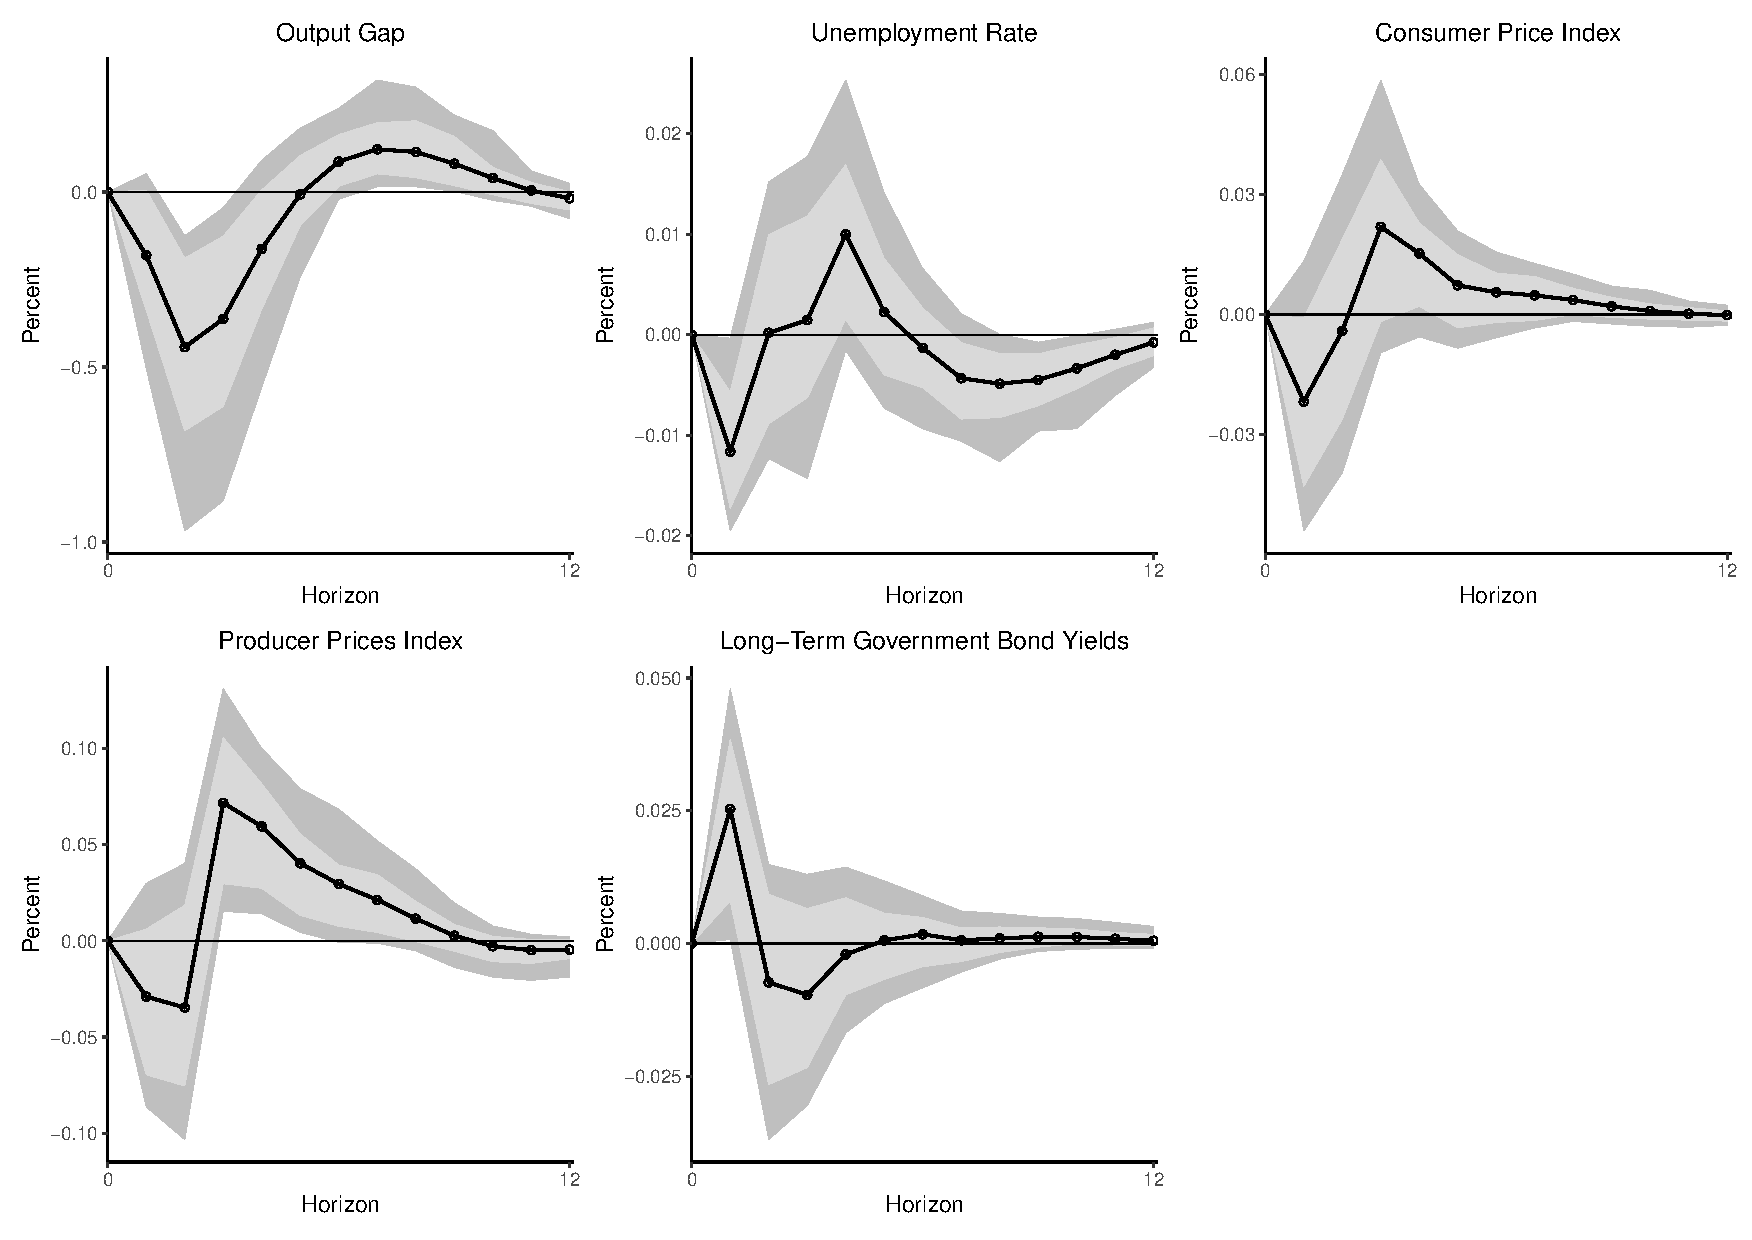
\includegraphics[width=\textwidth]{images/irf_lm.pdf}
    \caption*{Impulse Response from a sentiment index shock (LM-SA). The variables are described as follows: Output gap -- obtained from a HP filter from Real Gross Domestic Product (Euro/ECU series) for Euro area; Unemployment Rate -- Harmonized Unemployment Rate: Total: All Persons for the Euro Area}
    \label{fig:irflm}
\end{figure}


\begin{figure}
    \centering
    \caption{Impulse Response of a Sentiment Index (VADER) Shock on Economic Activity}
    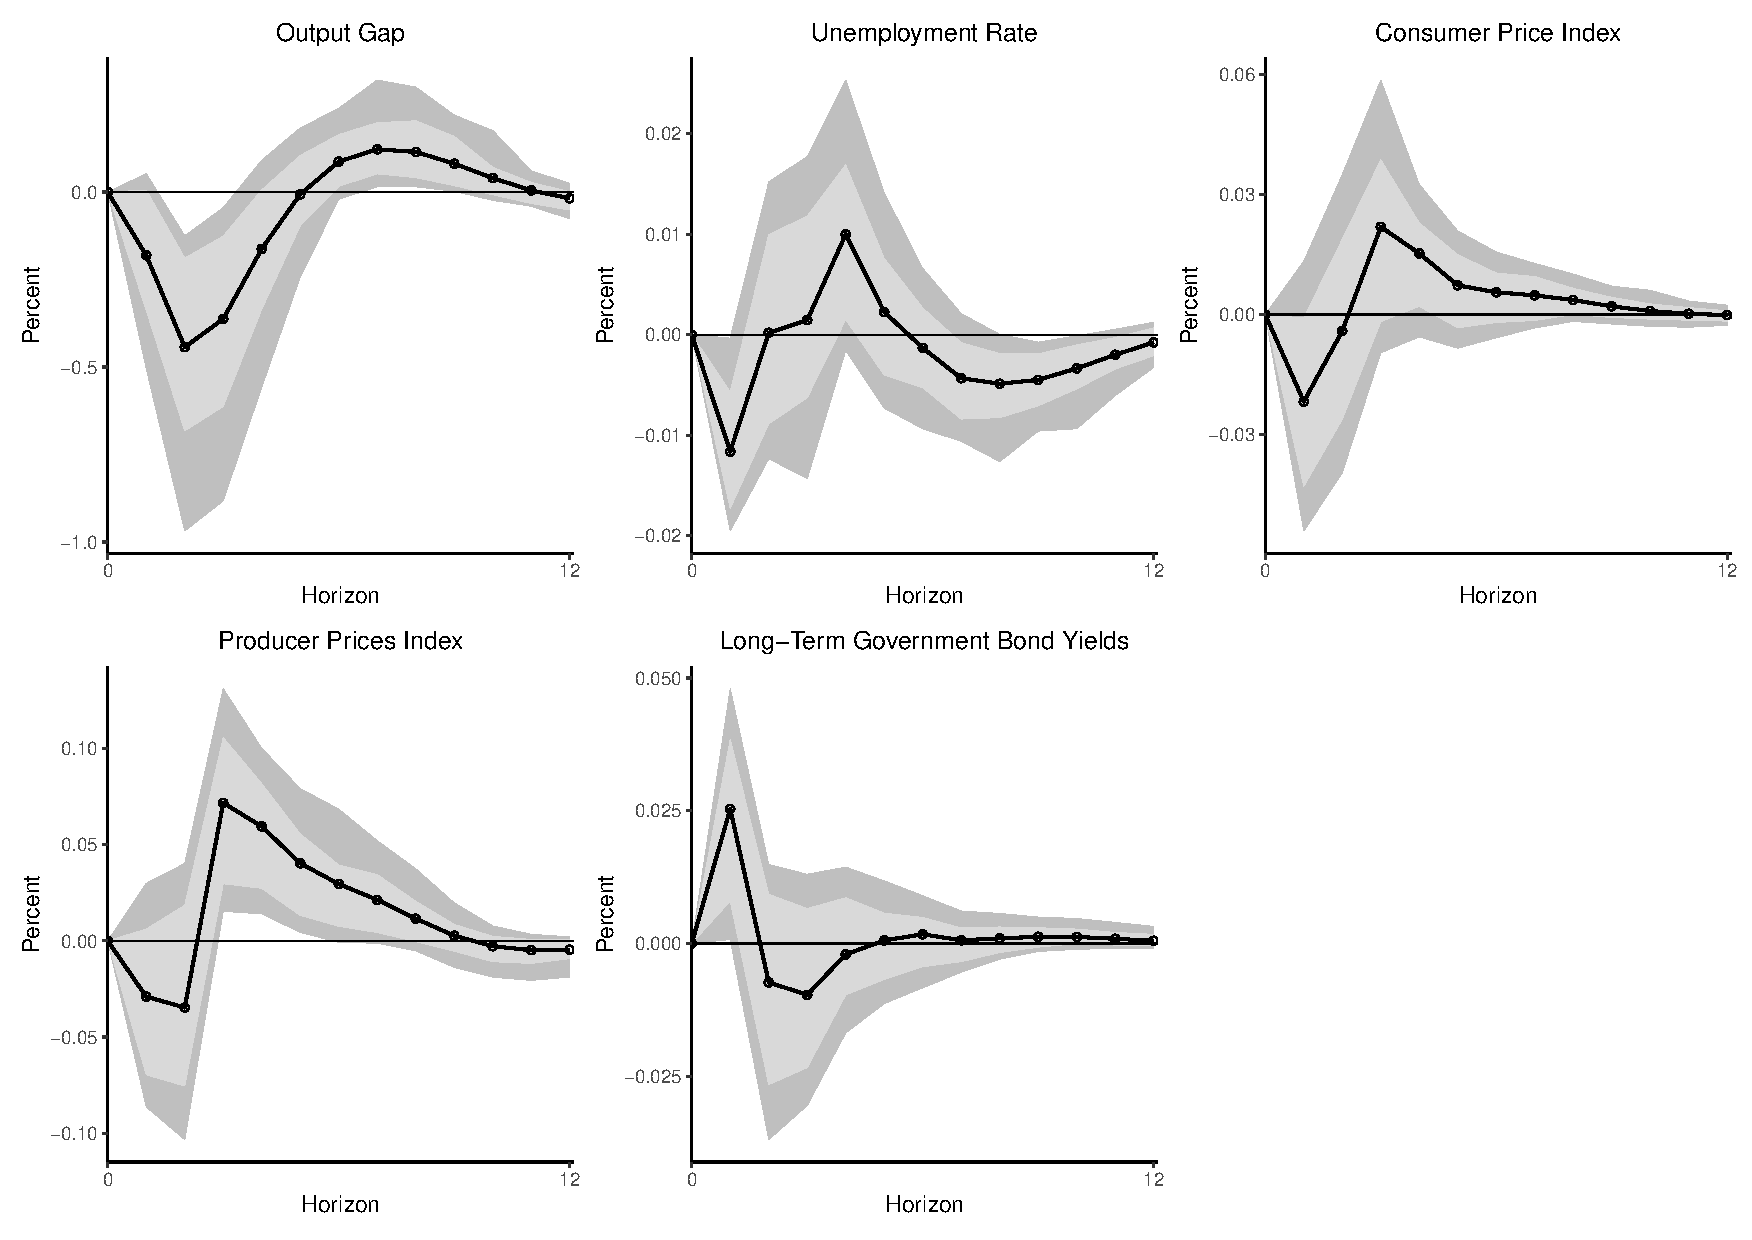
\includegraphics[width=\textwidth]{images/irf_lm.pdf}
    \caption{Caption}
    \label{fig:my_label}
\end{figure}

\section{Discussion}
